\chapter{Results}
% - Present the newly designed web-based acoustic event classification model.

\section{Demonstration of the Web-Based Model}
% - Discuss how the redesign enhances user-friendliness and accessibility.
% - Include user feedback or case studies.


\subsection{System Architecture and Implementation}
% - Detailed walkthrough of the backend and frontend setup
% - Explanation of the docker compose environment, Eclipse Mosquitto, Prometheus, Grafana, Alertmanager, Nginx, and Traefix proxy
% - Description of the MQTT-exporter and its integration with Prometheus
This section provides a comprehensive demonstration of our web-based result, focusing on both the backend and frontend implementations, as well as the setup of the supporting infrastructure.

\subsubsection{Backend Architecture}
The core of the system is a robust backend server responsible for device management, alert management, and providing an API for reloading \textsc{Prometheus} alert rules. The MQTT-exporter, designed to record classifier results and expose them to \textsc{Prometheus} in a format compatible with \textsc{Prometheus} runs soundly and safely.

\begin{figure}[htbp]
  \centering
  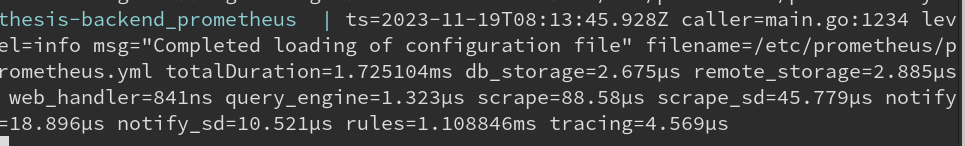
\includegraphics[width=0.85\textwidth]{Pictures/prometheusreload}
  \caption{\label{fig:prometheusreload}\textsc{Prometheus} successfully reload when the API is called properly}
\end{figure}

\subsubsection{Infrastructure Setup}
The system operates within a \textsc{Docker Compose} environment, in an isolated network namespace, ensuring security, scalability, and ease of deployment. The services running include our backend APIs, \textsc{Eclipse Mosquitto} with file-based user and access control list (ACL) management, \textsc{Prometheus}, \textsc{Grafana} and \textsc{mosquitto-exporter} exposing metrics to \textsc{Prometheus} for comprehensive monitoring.

\begin{figure}[htbp]
  \centering
  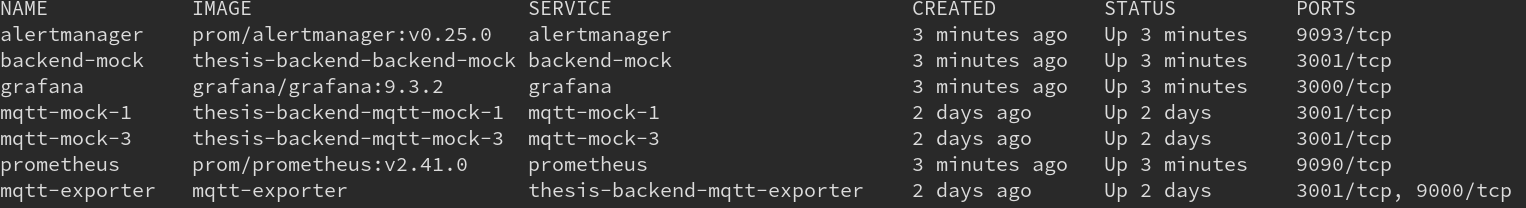
\includegraphics[width=0.85\textwidth]{Pictures/dockerps}
  \caption{\label{fig:dockerps}Running \textsc{Docker} Services}
\end{figure}

\subsubsection{Frontend Interface}
The frontend is deployed statically and is served by \textsc{Nginx}. \textsc{Bootstrap v5} is employed for styling, emphasizing accessibility and a user-friendly interface. The application showcases a single-page layout for streamlined user interaction. Additionally, intuitive interfaces are provided for managing devices and alerts.

\begin{figure}[htbp]
  \centering
  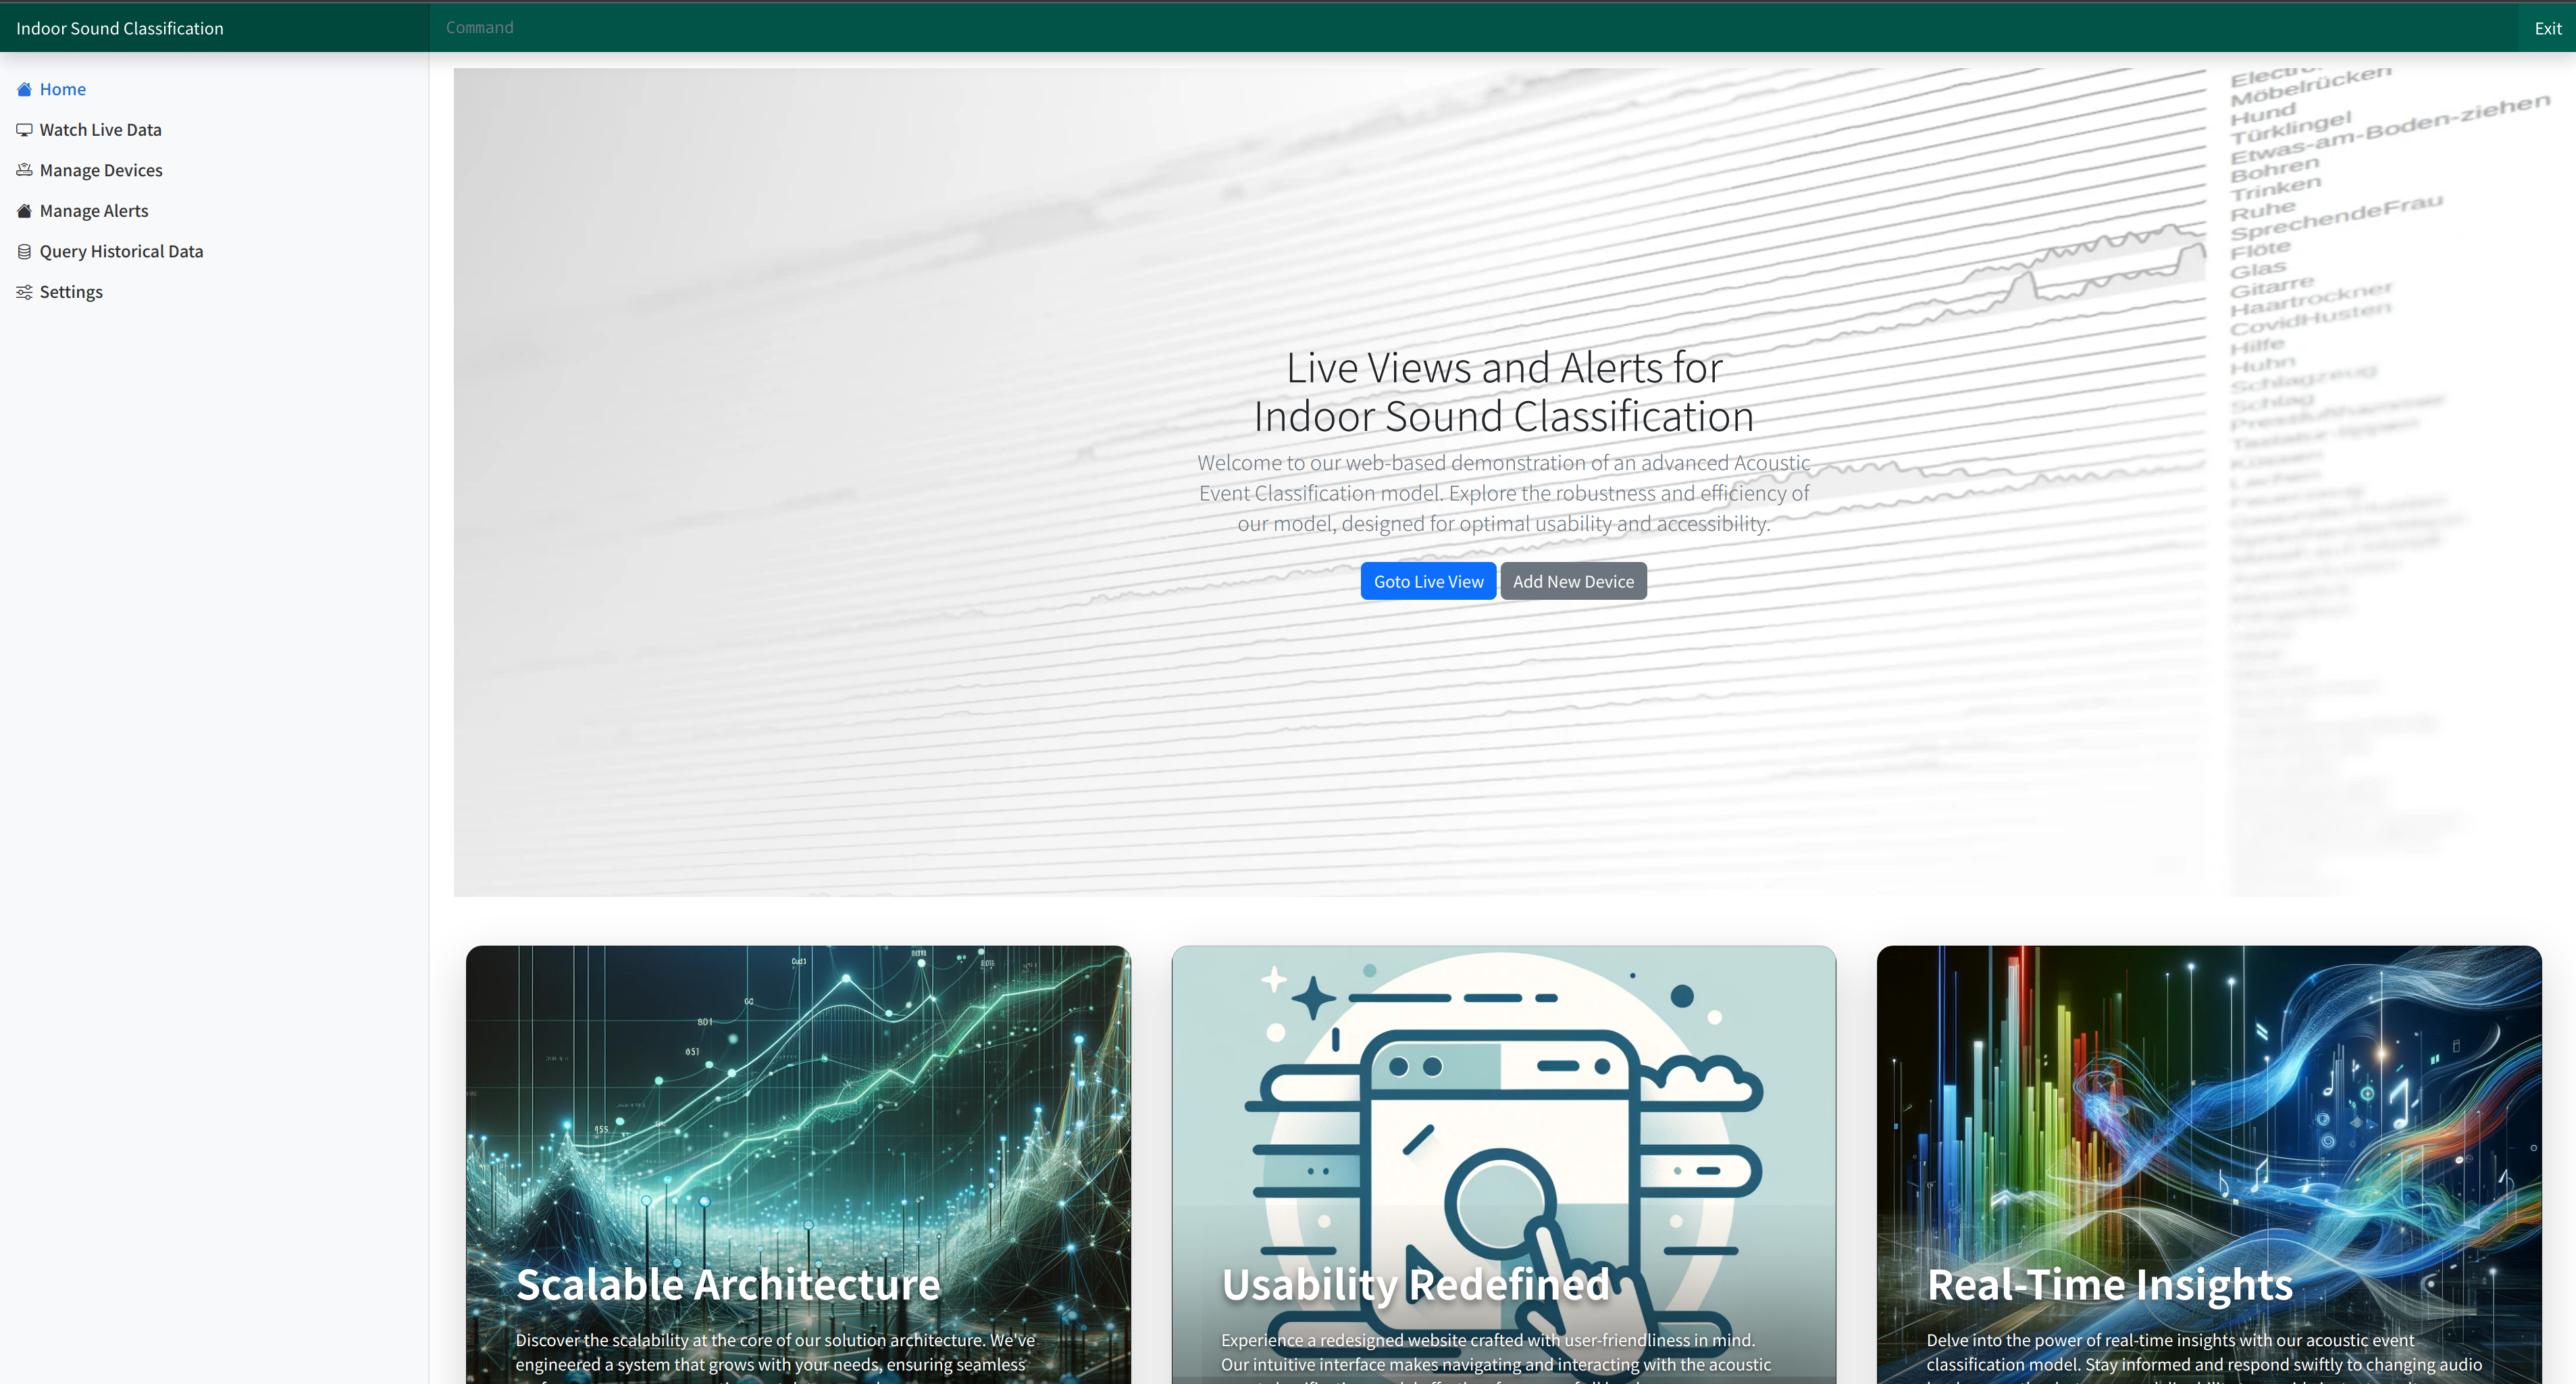
\includegraphics[width=0.85\textwidth]{Pictures/home}
  \caption{\label{fig:schome}Landing Page Design}
\end{figure}

\subsubsection{Data Visualization and Management Interfaces}
The live view feature subscribes to the MQTT server, presenting a real-time data stream from the acoustic event classifier. This data is rendered in a heatmap format, with the last 60 seconds on the X-axis and classification tags on the Y-axis. The color intensity represents the confidence level of predictions.

% Insert Screenshot: Live View and Heatmap Visualization]


\subsection{Frontend Interface and Features}
% - Overview of the single-page web application built with ReactJS
% - Description of key features:
%   - Live view subscribing to MQTT server
%   - Heatmap visualization of real-time data
%   - Interfaces for classifier and alert management
%   - Historical data visualization and server credential settings

\subsubsection{Single Page Web Application}
A streamlined, single-page application allows for real-time monitoring and management without the need for reloading or navigating multiple pages.

\subsubsection{Heatmap Visualization}
The innovative heatmap visualization offers a quick and intuitive understanding of the classifier's real-time output. The visualization uses time (last 60 seconds) as the X-axis and classification tags as the Y-axis, with varying color intensities indicating prediction confidence.

\begin{figure}[htbp]
  \centering
  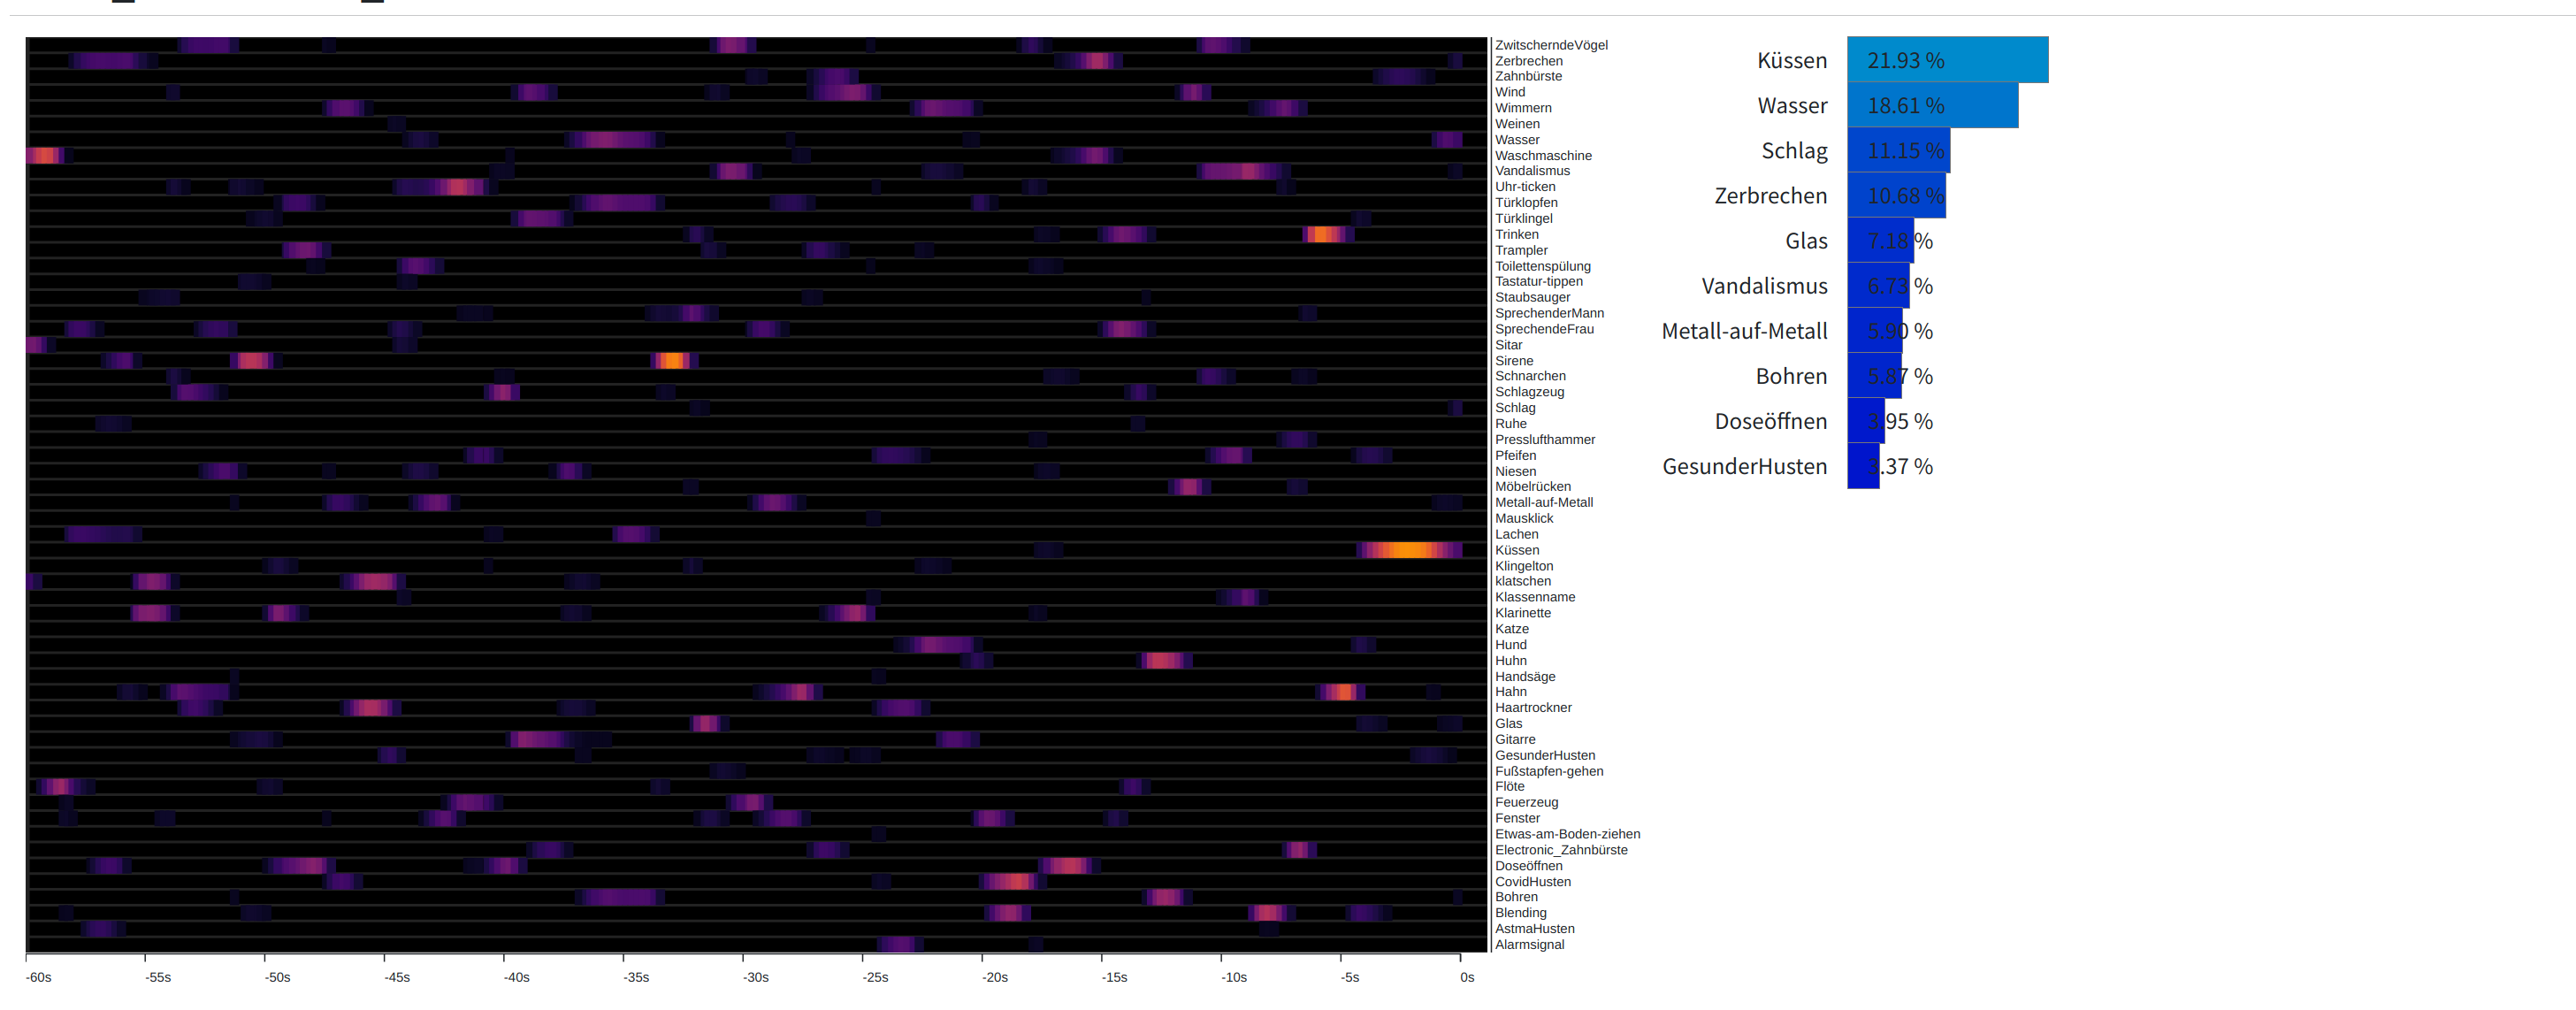
\includegraphics[width=0.85\textwidth]{Pictures/heatmap}
  \caption{\label{fig:heatmap}Live Streaming Data Visualization}
\end{figure}

\subsubsection{Classifier and Alert Management}
The interfaces for managing classifiers and alerts are designed for ease of use, allowing users to seamlessly control and configure the system according to their specific needs.

\begin{figure}[htbp]
  \centering
  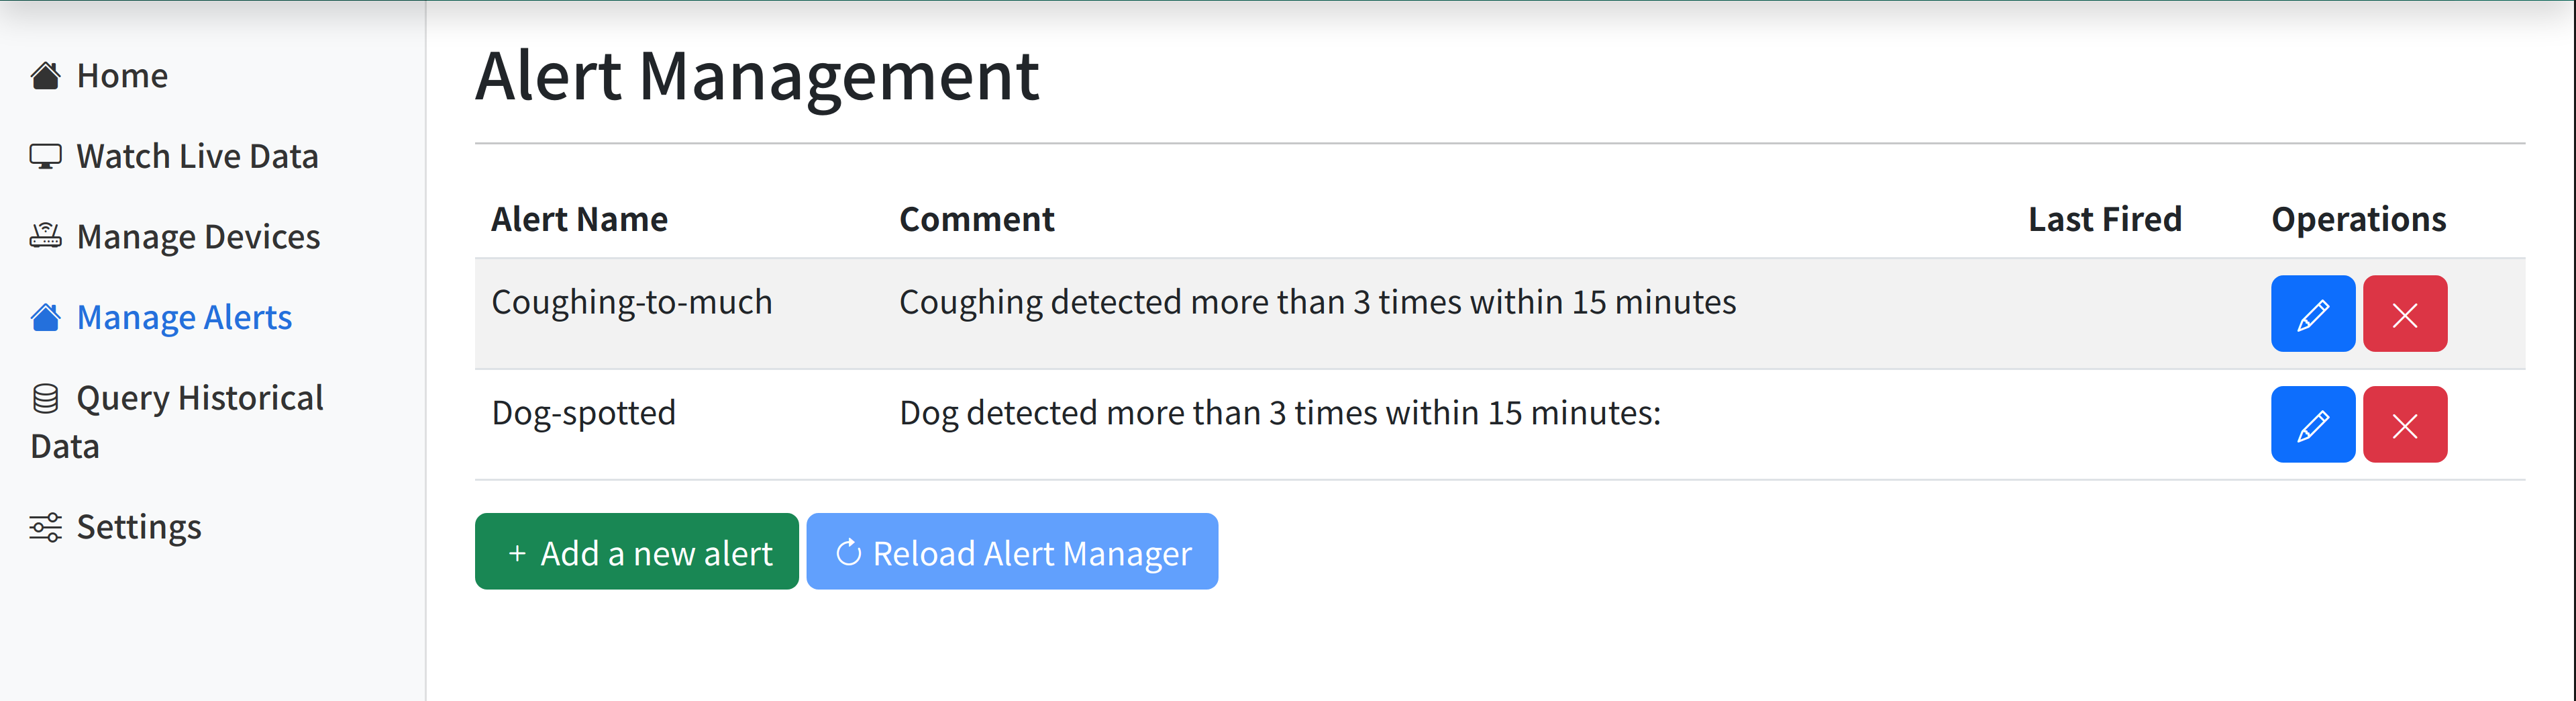
\includegraphics[width=0.85\textwidth]{Pictures/alertmanagement}
  \caption{\label{fig:alertmanagement}Alert Management Interface}
\end{figure}

\begin{figure}[htbp]
  \centering
  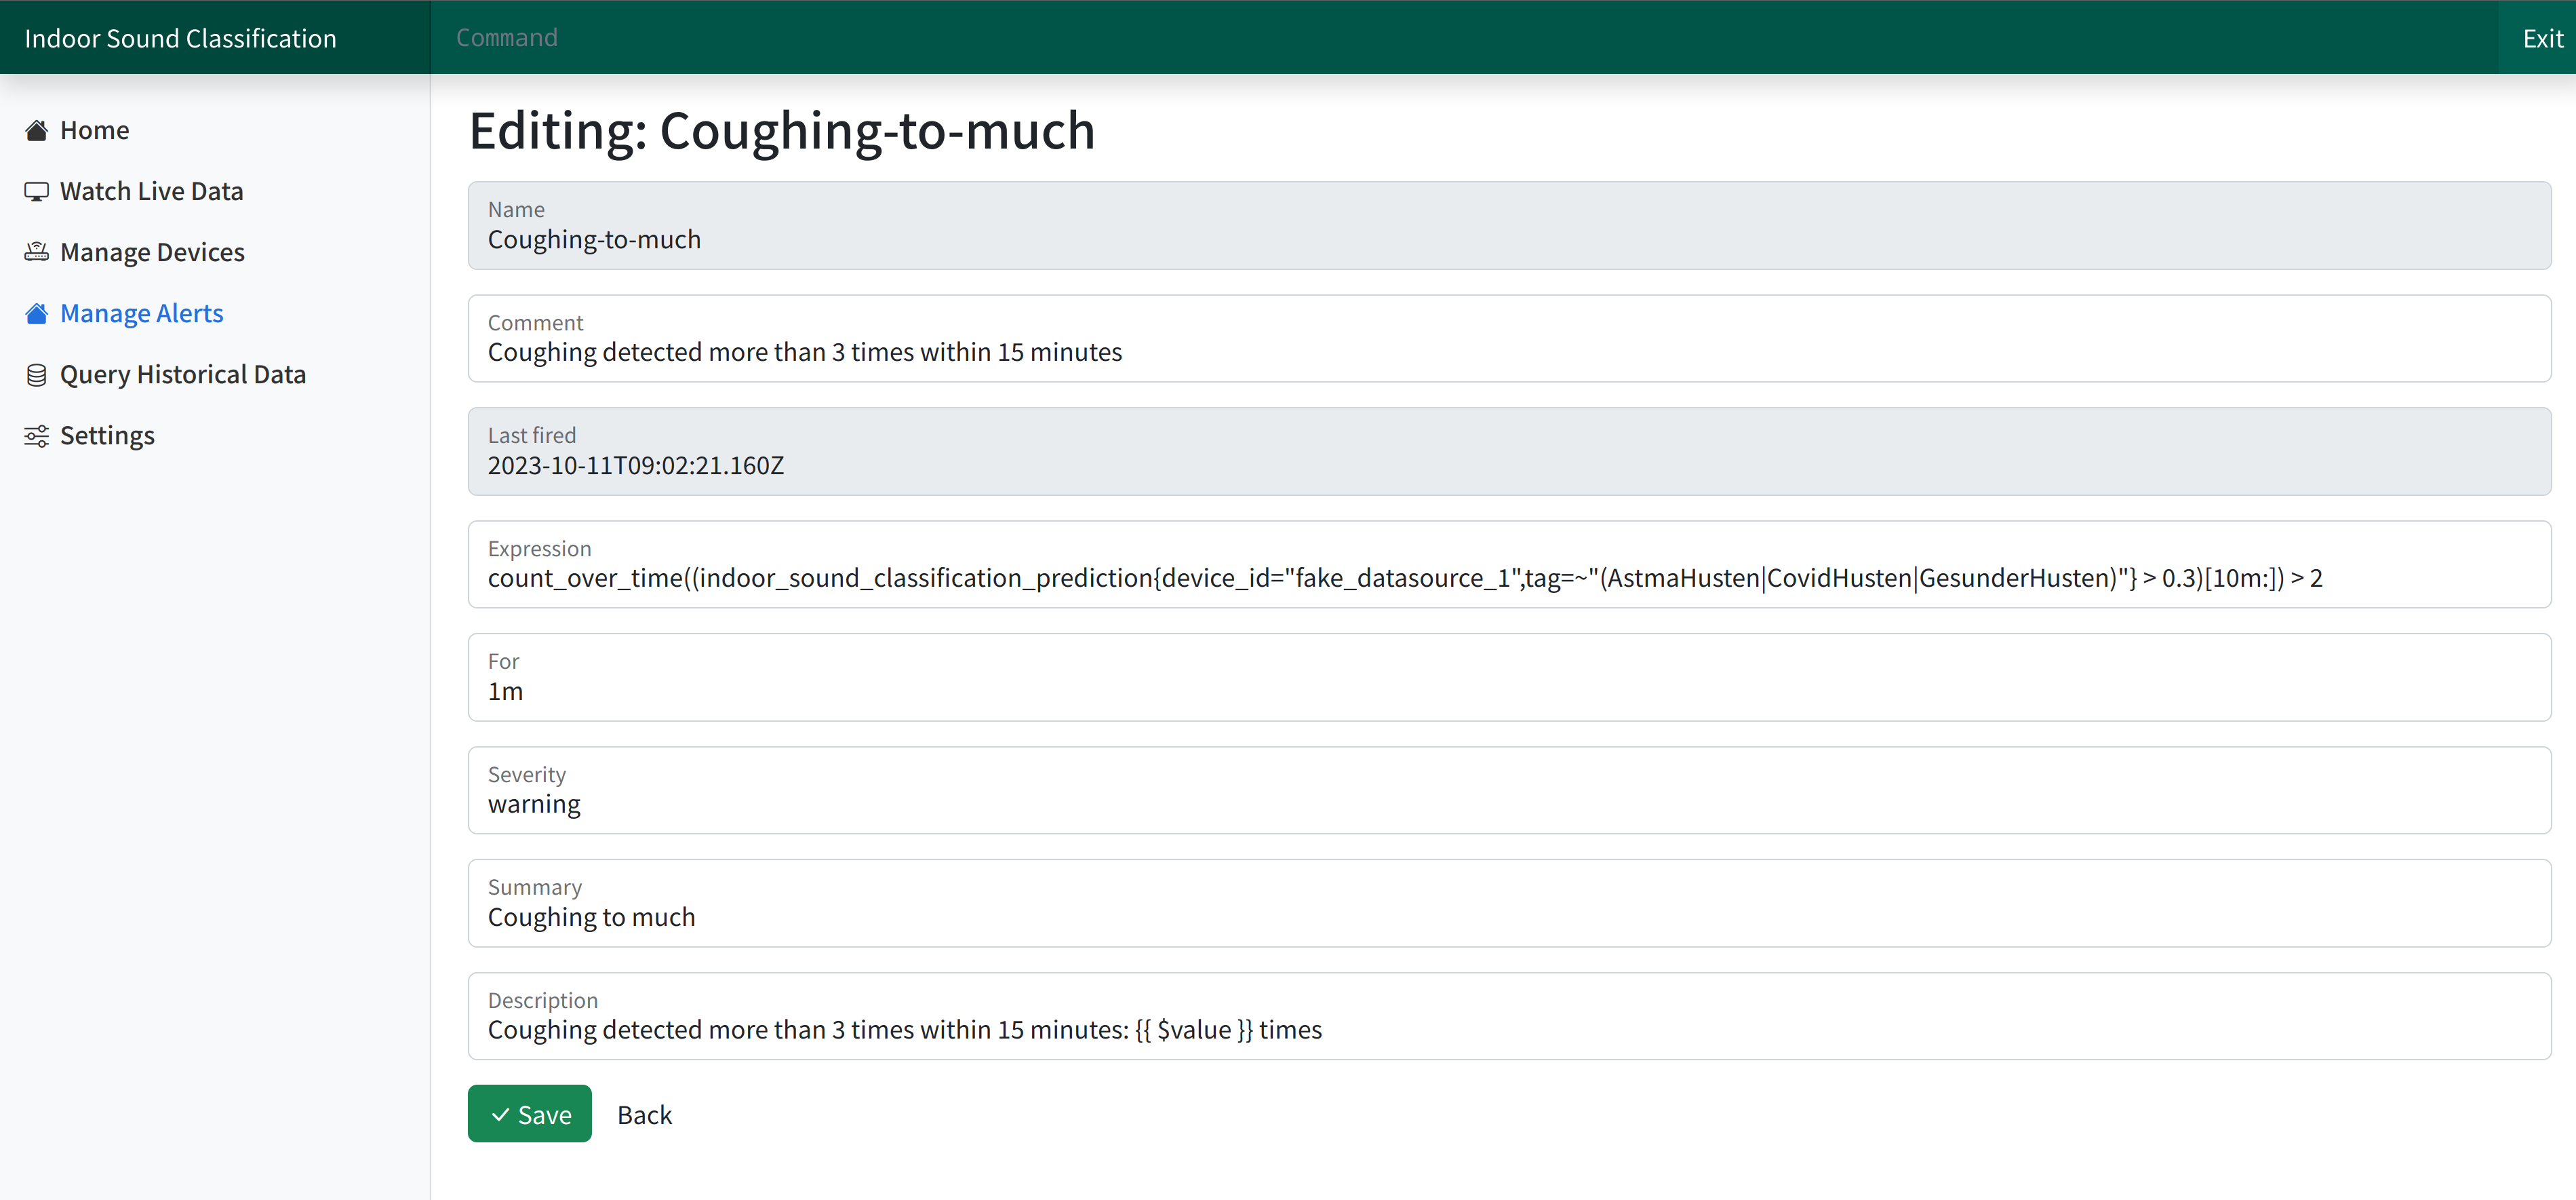
\includegraphics[width=0.85\textwidth]{Pictures/alertedit}
  \caption{\label{fig:alertedit}Alert Editing Interface}
\end{figure}

\subsubsection{Settings and Configuration}: A dedicated settings page is included for users to easily input and update server credentials, ensuring secure and personalized access to the system.

\subsubsection{Historical Data Visualization}
The application also provides various visualizations of historical data, extracted from \textsc{Prometheus} TSDB via \textsc{Grafana}, aiding in long-term analysis and trends observation.

\begin{figure}[htbp]
  \centering
  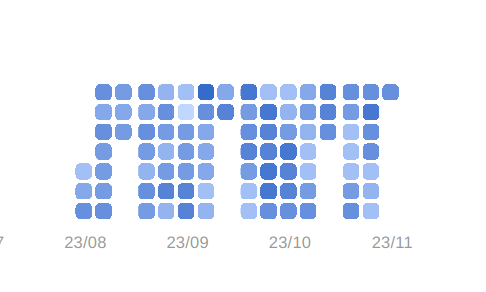
\includegraphics[width=0.85\textwidth]{Pictures/calendar-weekday-day}
  \caption{\label{fig:calendar-weekday-day}Calendar View of Event Frequencies}
\end{figure}
\subsubsection{Settings and Configuration}: A dedicated settings page is included for users to easily input and update server credentials, ensuring secure and personalized access to the system.

\begin{figure}[htbp]
  \centering
  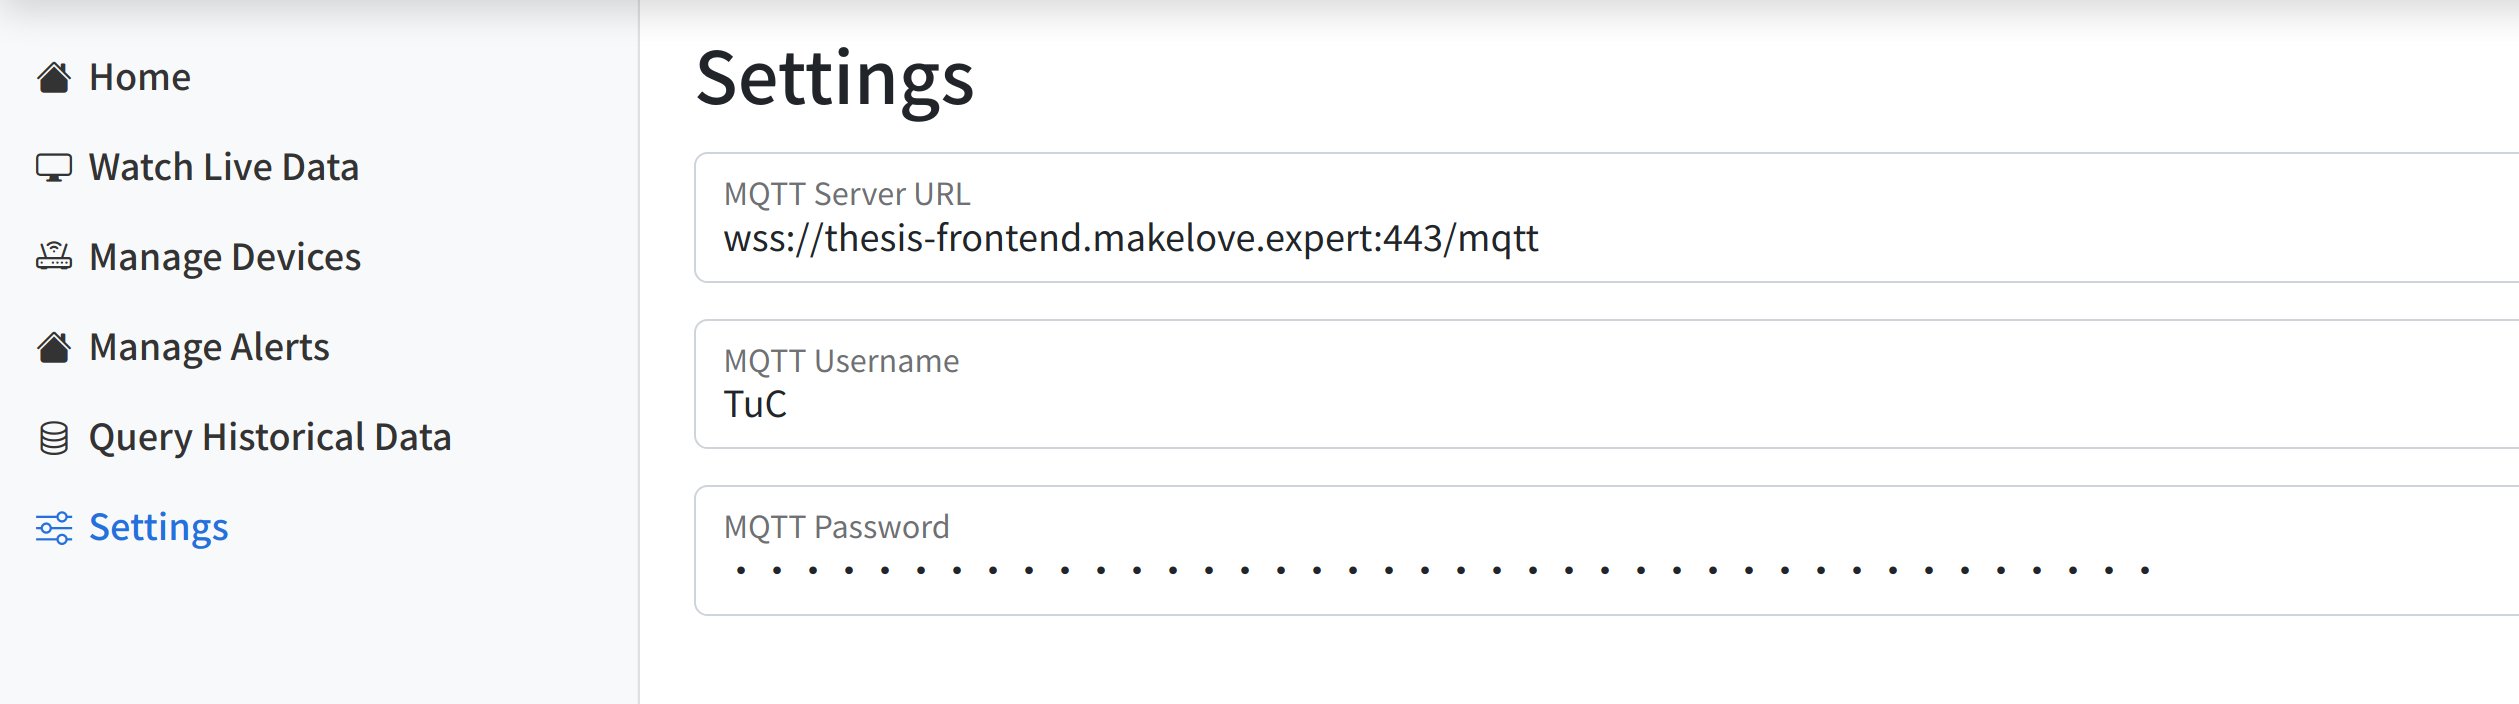
\includegraphics[width=0.85\textwidth]{Pictures/settings}
  \caption{\label{fig:settings}Settings Interface}
\end{figure}


In summary, the web-based model demonstrates a cohesive integration of backend robustness with frontend accessibility, underpinned by a user-friendly interface and effective data visualization techniques. The system architecture not only addresses the technical requirements of acoustic event classification but also emphasizes the importance of user experience and accessibility.

\section{Testing of the Alert System}
% - Simulation tests to assess the effectiveness of the alert system, including the responsiveness and accuracy of email alerts.
% - Performance analysis of the alert manager in various simulated emergency scenarios.
\subsection{Test Setup and Methodology}
In order to evaluate the effectiveness and reliability of the alert system, a comprehensive testing strategy is implemented. The test environment is configured to mimic real-world conditions as closely as possible. This involves setting up the complete system architecture, including the backend server, MQTT-exporter, and the integration with \textsc{Prometheus} and \textsc{Alertmanager}.

The methodology involves generating a series of simulated acoustic events, which are then classified and processed by the system. These events are designed to test the system's ability to accurately detect and categorize different types of acoustic signals, and subsequently trigger appropriate alerts.

We use Perlin noise to simulate acoustic events. The predictions of the classifier are broadcasted by \textsc{Mosquitto} and the MQTT-exporter records the result. \textsc{Prometheus} scrapes the result from MQTT-exporter and evaluates the alert rules, and in the end triggers the \textsc{Alertmanager} to send alerts by email.

\subsection{Test Results}
\subsubsection{Alert Triggering}
The tests showed that the alerts are successfully triggered under specific conditions designed to mimic real acoustic events. For instance, when a predefined sound pattern is detected, the system promptly identifies it and triggers the corresponding alert. This demonstrates the system's ability to react accurately to environmental cues.

\subsubsection{Alert Rules Evaluation Time}

A critical aspect of the alert system's performance is the speed of alert rule evaluation. During testing, the average alert rules evaluation time is measured to be approximately 145 milliseconds. This quick response time is essential in situations where timely alerts are crucial, and it underscores the system's efficiency.

% screenshot alert rules evaluation time

\subsubsection{Email Notification Delivery}
The effectiveness of the alert system also depends on the successful delivery of notifications. In this regard, the system performed admirably. Emails generated as a result of the triggered alerts are sent and successfully delivered to the recipient's mailboxes. This is verified through a combination of automated scripts and manual checks. The emails contain detailed information about the alert, including the time of occurrence and the specific nature of the acoustic event.

\begin{figure}[htbp]
  \centering
  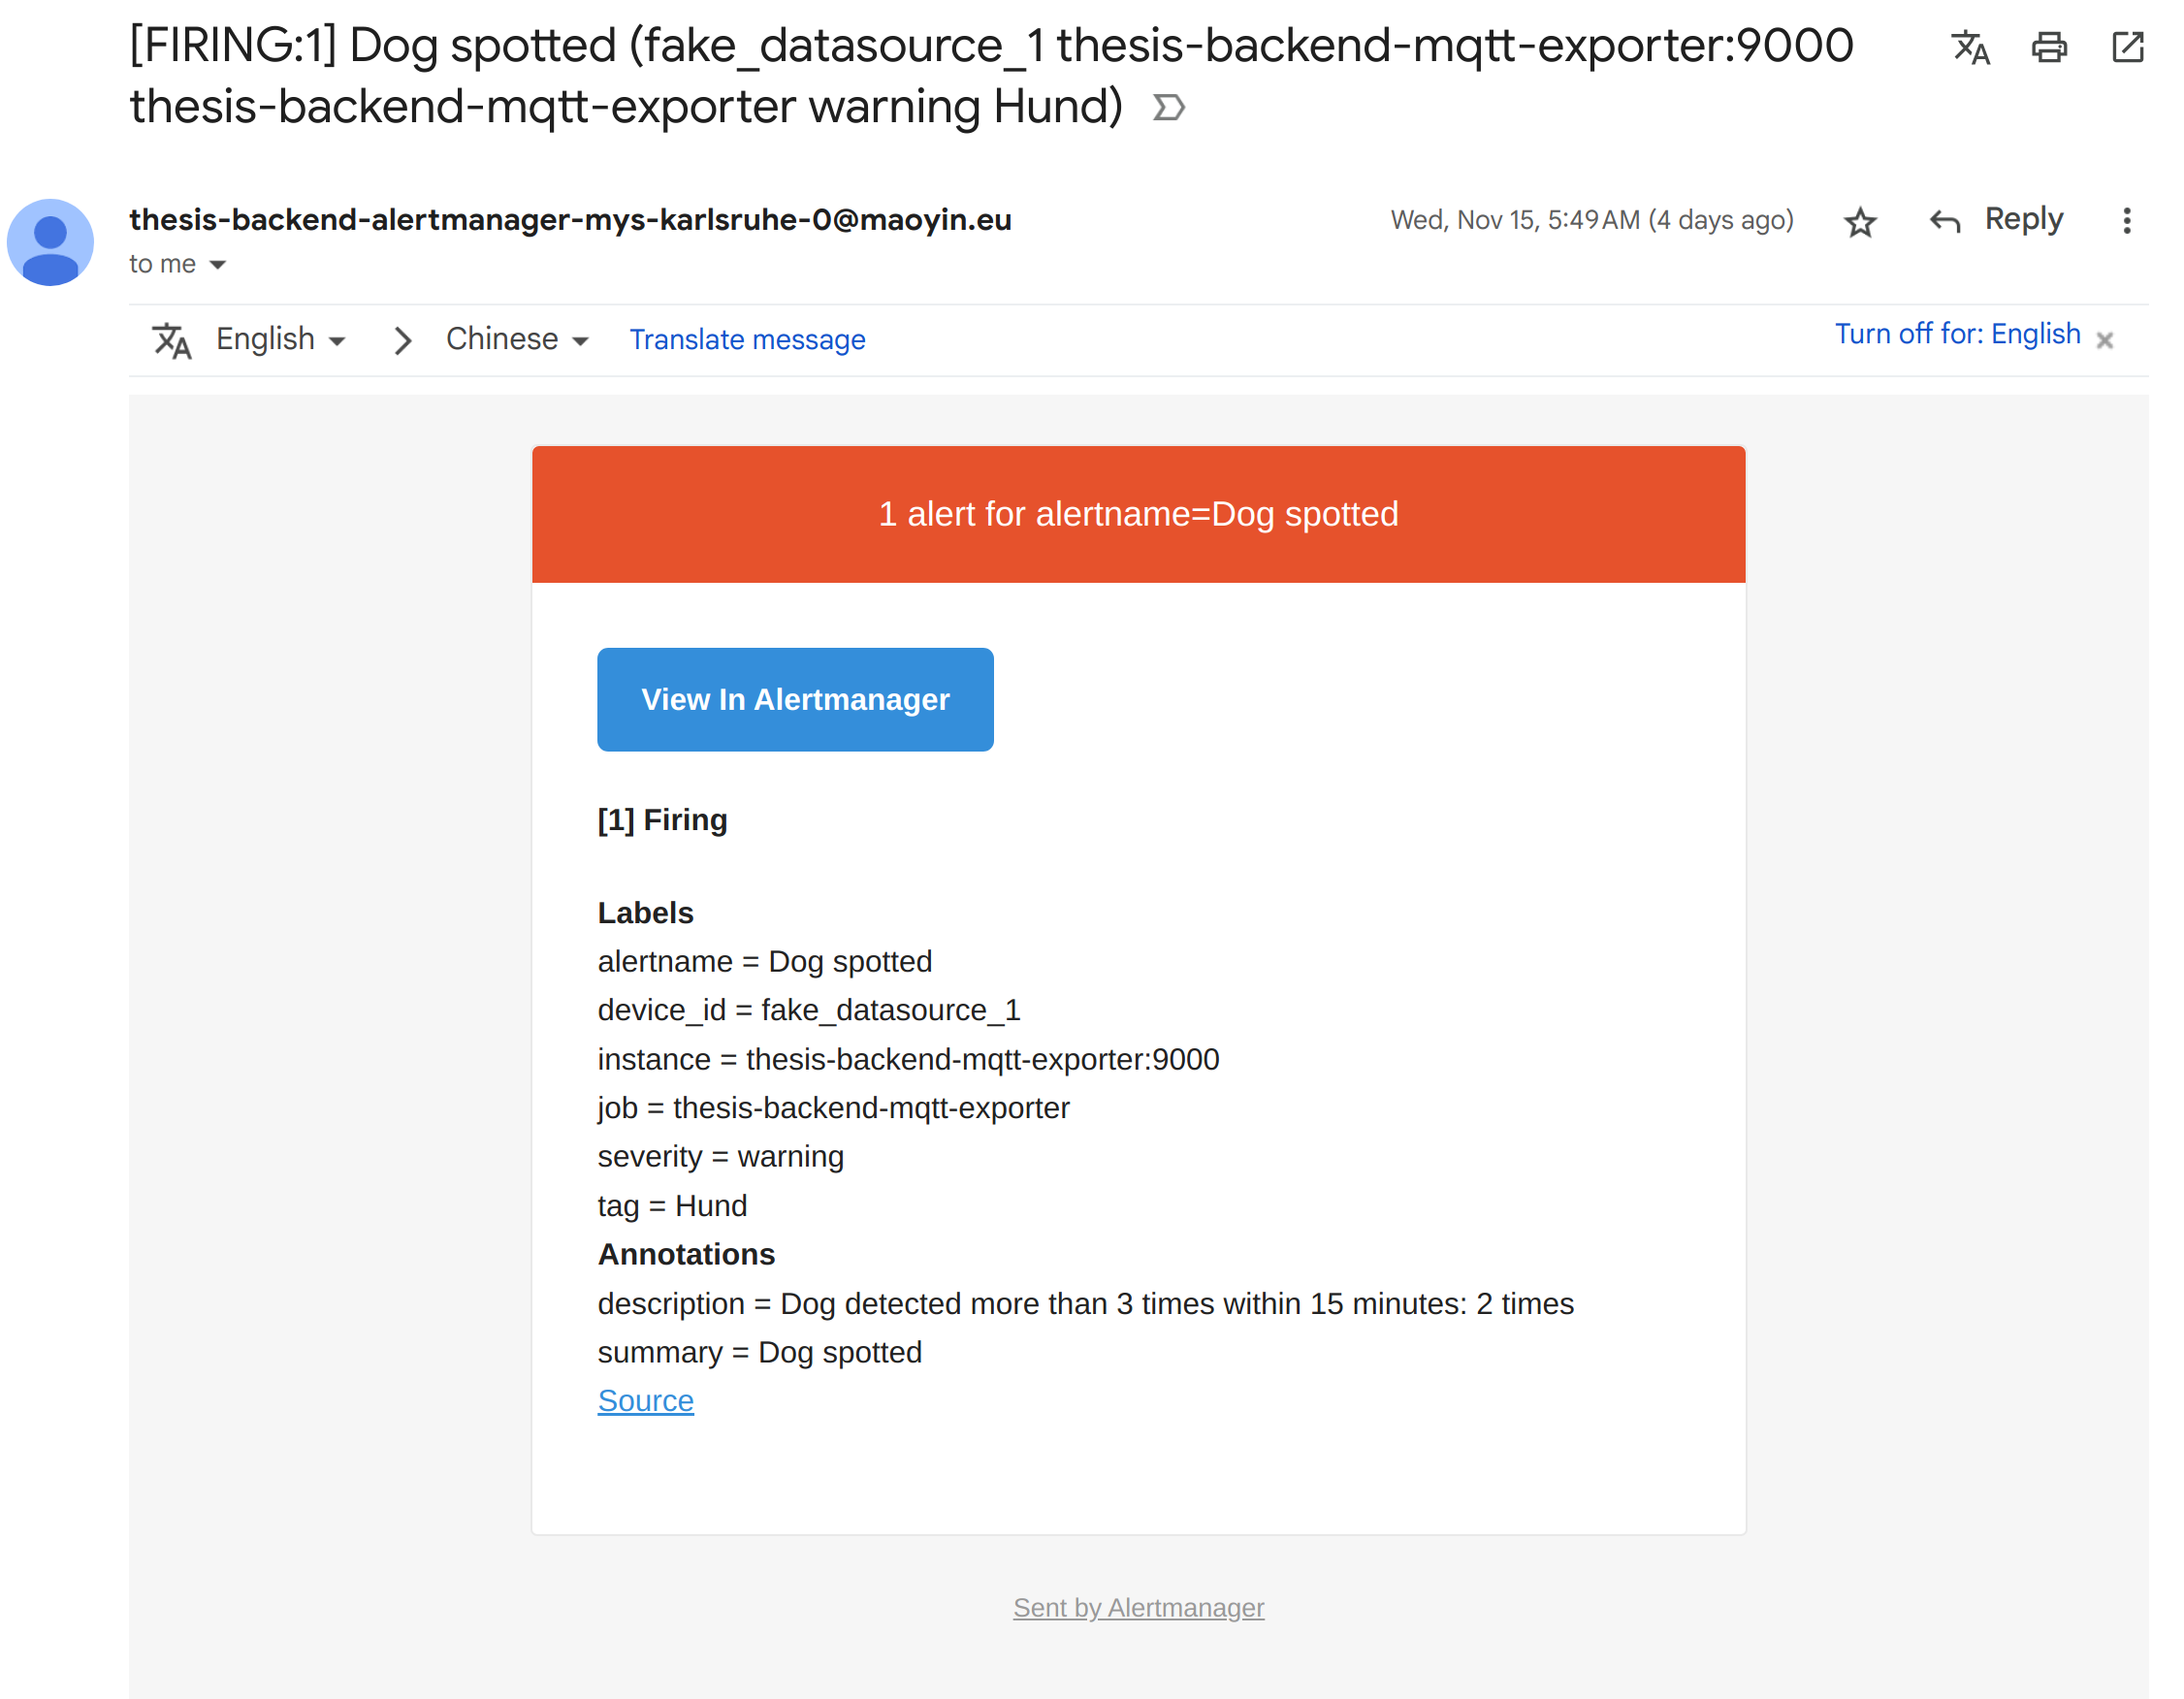
\includegraphics[width=0.85\textwidth]{Pictures/email}
  \caption{\label{fig:email}The Delivered Alert Email}
\end{figure}

The tests conducted on the alert system have conclusively demonstrated its reliability and efficiency. The system's ability to promptly trigger alerts, quickly evaluate alert rules, and effectively deliver email notifications, all within a fraction of a second, speaks to its robustness and practicality in real-world applications. These results are a testament to the successful implementation of the alert system within the broader framework of the acoustic event classification model.

\section{User-Friendliness and Accessibility}
% - Present the results of usability and accessibility testing.
% - Discuss how the web-based solution fulfills these aspects.
\subsubsection{Web Accessibility Evaluation}
The web application is rigorously evaluated for accessibility using a range of Web Accessibility Evaluation Tools. These tools assess key areas such as screen reader compatibility, keyboard navigation, and adherence to the Web Content Accessibility Guidelines (WCAG).

\subsubsection{Evaluation Results}
\begin{itemize}
  \item \textbf{Screen Reader Compatibility}: The application is tested with several leading screen readers. Results indicated high compatibility, with screen readers effectively interpreting and voicing out content and navigation elements.
  \item \textbf{Keyboard Navigation}: The application supports comprehensive keyboard navigation. Testing shows that users can navigate through all interactive elements using the keyboard, a vital feature for users with motor impairments or those who prefer keyboard inputs.
  \item \textbf{Color Contrast and Text Readability}: The evaluation tools checked for color contrast ratios and text readability. The application meets the recommended contrast ratios, ensuring that text is legible and distinguishable for users with visual impairments.
  \item \textbf{ALT Tags and ARIA Labels}: The usage of ALT tags for images and ARIA labels for interactive elements is found to be consistent and descriptive, aiding users who rely on assistive technologies to understand and interact with the content.
  \item \textbf{Responsive Design}: The application's responsive design is tested across various devices and screen sizes. This ensures accessibility and usability irrespective of the device used, accommodating users with different preferences and requirements.
\end{itemize}

\subsubsection{Compliance with WCAG}
The evaluation results indicate that the application adheres to the WCAG guidelines, specifically meeting criteria for levels A and AA. This compliance underscores the application's commitment to being accessible to a broad spectrum of users, including those with disabilities.

Overall, the accessibility features integrated into the application demonstrate a strong commitment to inclusivity. The results from the Web Accessibility Evaluation Tools affirm that the design choices effectively cater to users with diverse needs and preferences, making the application a model for accessible web design in the context of acoustic event classification.

\section{Feedback Analysis}
\subsection{Feedback Collection}
% - Explanation of the method used for collecting machine-based feedback
In order to evaluate the performance and efficiency of our web-based acoustic event classification demonstration system, we utilized a suite of machine-based analysis tools. These included:

\begin{itemize}
  \item \textbf{Web Vitals}: To measure the user experience and performance metrics of the web application.
  \item \textbf{Chrome Developer Tools (DevTools)}: Utilized for profiling the application, generating flame graphs and heap snapshots to understand resource consumption and potential bottlenecks.
  \item \textbf{stat.js}: Integrated for real-time monitoring of render time consumption, frames per second (FPS), and memory usage, providing a continuous feedback loop during the development and usage phases.
\end{itemize}

\subsection{Analysis of Web Vitals}
Web Vitals provided valuable insights into the user experience, particularly focusing on metrics such as Largest Contentful Paint (LCP), First Input Delay (FID), and Cumulative Layout Shift (CLS). These metrics helped in identifying areas where the application's performance could be optimized for a smoother and more responsive user experience.

\begin{table}[h!]
  \centering
  \begin{tabular}{|r|l|l|}
    \hline
    Name & Delta              & Rating \\ [0.5ex]
    \hline\hline
    FID  & 2.199999988079071  & Good   \\
    \hline
    FCP  & 502.69999998807907 & Good   \\
    \hline
    TTFB & 22.099999994039536 & Good   \\
    \hline
    CLS  & 0.0                & Good   \\
    \hline
    LCP  & 918.4000000059605  & Good   \\[1ex]
    \hline
  \end{tabular}
  \caption{\label{table:webvitals}Web Vitals Report}
\end{table}


\subsection{Profiling with Flame Graphs and Heap Snapshots}
The profiling of the application using DevTools is instrumental in pinpointing specific areas where the application's performance can be improved. Flame graphs offer a visual representation of the execution time of various functions, aiding in identifying performance bottlenecks. Heap snapshots provide an in-depth look at memory usage, which is critical in detecting memory leaks and optimizing memory management.

\begin{figure}[htbp]
  \centering
  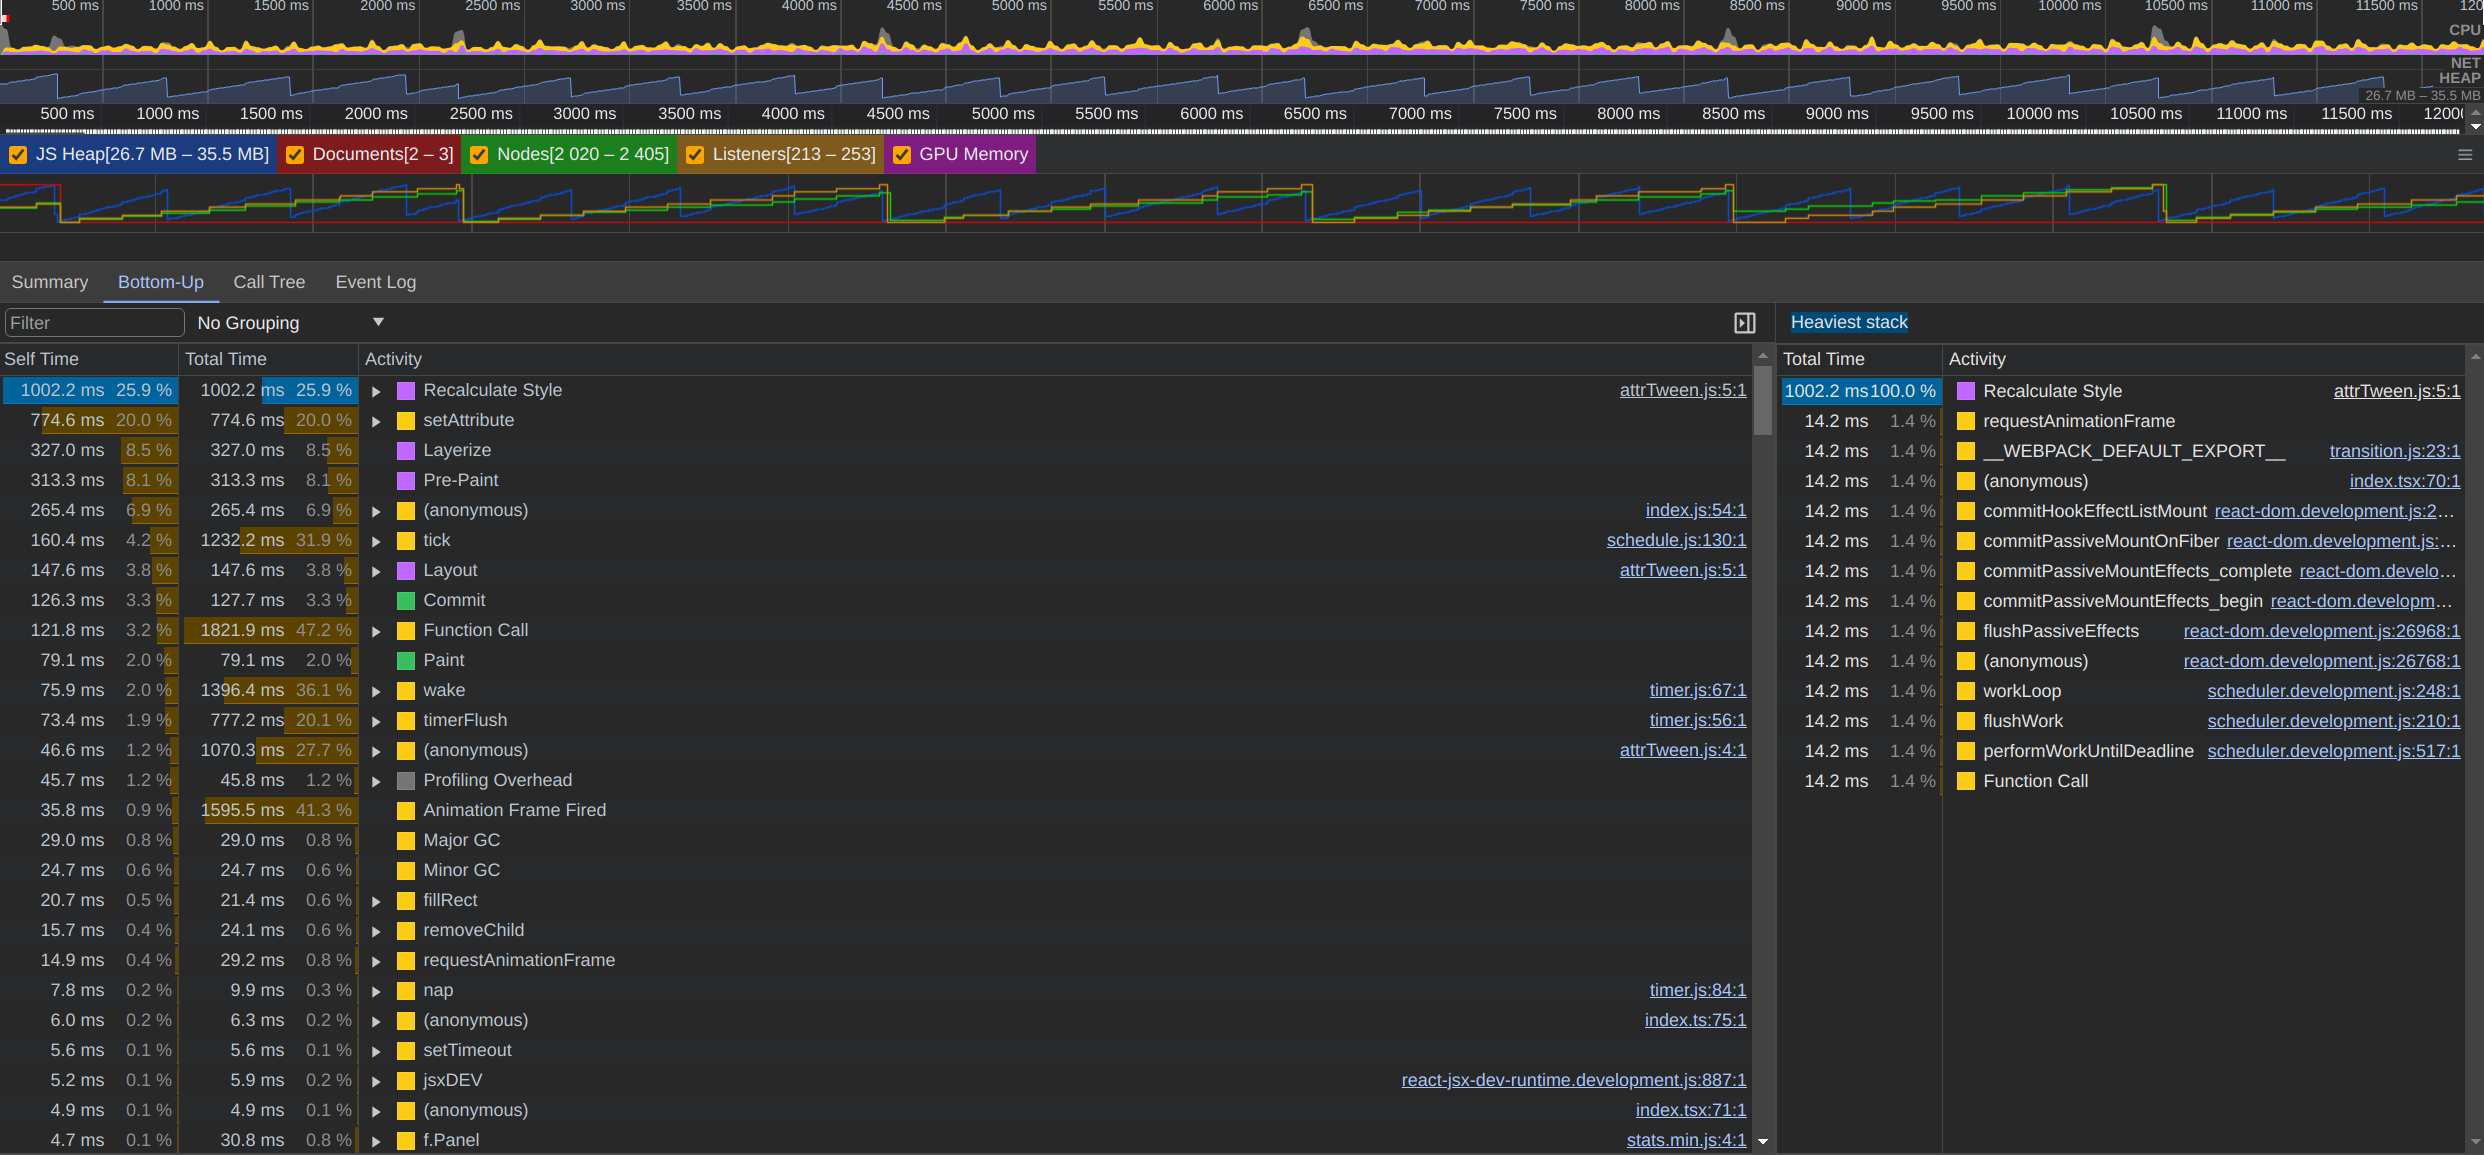
\includegraphics[width=0.85\textwidth]{Pictures/profiling}
  \caption{\label{fig:profiling}The Profiling of Around 10 Seconds Sample}
\end{figure}
\subsection{Real-Time Monitoring with \textsc{Stat.js}}
\textsc{Stat.js} is employed to monitor the system's performance in real-time, specifically focusing on render time, FPS, and memory usage. This continuous monitoring allows for the immediate detection and resolution of issues that arise during the application's operation, ensuring optimal performance at all times. The render time and FPS metrics are particularly useful in evaluating the efficiency of the visualization components, such as the heatmap and live data stream renderings.

\begin{figure}[htbp]
  \centering
  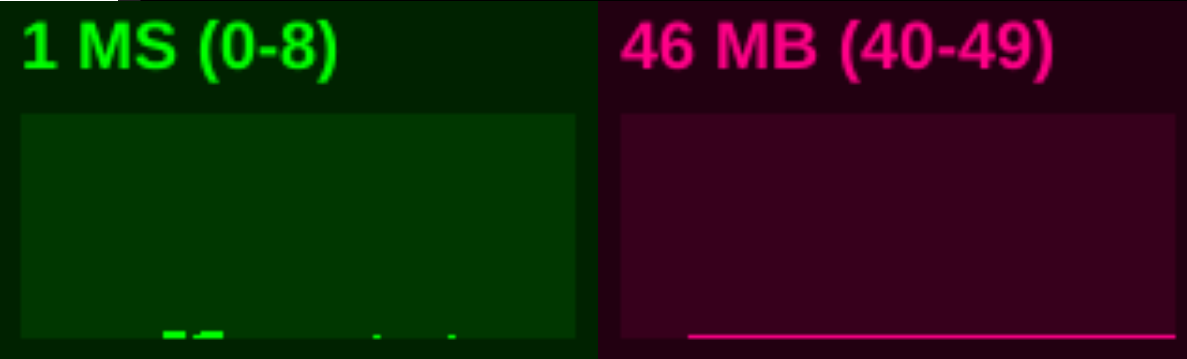
\includegraphics[width=0.85\textwidth]{Pictures/stats}
  \caption{\label{fig:stats}Timing and Memory Usage of the Visualization}
\end{figure}

The machine-based feedback analysis provides a comprehensive overview of the system's performance from a technical standpoint. The insights gathered from Web Vitals, flame graphs, heap snapshots, and \textsc{Stat.js} metrics are integral in refining the application, ensuring it not only meets but exceeds the standards of robustness, efficiency, and user experience.
